%!TeX ts-program = xelatex
%!TeX encoding = utf-8 Unicode
\documentclass[ieeetran]{article}
\usepackage{amsmath, amssymb}
\usepackage{graphicx}



\title{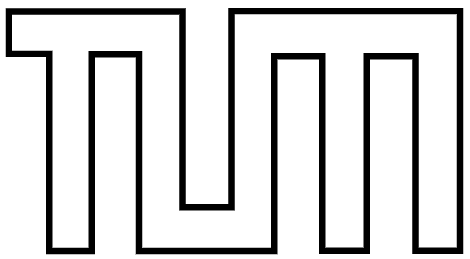
\includegraphics[width=0.43\textwidth]{tumlogo}\hspace{2ex}
\includegraphics[width=0.25\textwidth]{maxlogo}\vspace{1ex}\\ \large \textbf{Max Planck Computing and Data Facility \\Chair of Computer Architecture and Parallel Systems} \vspace{10ex}\\ \huge Tensorflow \vspace{2ex}\\
\large Seminar: Efficient Programming of HPC Systems \\Frameworks and Algorithms\vspace{15ex}}


\author{Efe Kamasoglu}


\begin{document}

\maketitle

\pagebreak

\tableofcontents

\pagebreak

\addcontentsline{toc}{section}{Abstract}
\section*{Abstract}



\pagebreak


\section{Introduction} % (fold)
\label{sec:introduction}
TensorFlow is a free and open-source framework developed by Google Brain, which finds its application widely in the field of machine learning and artificial intelligence. It is used to build and train large-scale models according to the client's preferences and provided data sets. In order to train a model, TensorFlow carries out several computations by mapping them onto a variety of hardware, such as mobile devices or systems consisting of multiple computational units with hundreds of GPUs. Those computations are represented in a "directed dataflow graph"\footnote{Martin Abadi, Ashish Agarwal, \ldots, "TensorFlow: Large-Scale Machine Learning on Heterogeneous Distributed Systems," November 9, 2015, p.\ 1, para.\ 2} as a whole, which is then compiled statically or dynamically depending on the version of Tensorflow \cite{first}. 
\\ \\To construct such graph, a client needs to create a session which is an interface with methods of its own. Through those methods, the client can introduce his data set to Tensorflow's system, define his model and its specifications. A graph is typically composed of the following \cite{first}:
\begin{itemize}
  \item \textit{Node:} A node has zero or more inputs and zero or more outputs. It is an instantiation of an operation.
\item \textit{Edge:} Data flows through the edges from one node to another. There are also edges which are not for the dataflow, but for control dependencies between different nodes; e.g., execution order of the concerning operations.
\item \textit{Operation:} An operation represents a computation such as addition or matrix dot product.
\item \textit{Tensor:} Tensors are multidimensional arrays describing the data. They flow into the nodes as inputs through the edges of a graph.
\item \textit{Kernel:} A kernel is an implementation of an operation.
\item \textit{Device:} Devices are computational units on a machine that are utilized by TensorFlow's system to execute kernels. (e.g.\ GPUs)
\end{itemize}
An example graph for a neural network is shown in Figure 1. $W, x$ are tensors which flow into 1.\ node with the operation $MatMul$ as inputs. Matrix multiplication of $W$ and $x$ is then computed and the result as well as tensor $b$ are fed into 2.\ node. Addition of those flow into 3.\ node, where the $ReLU$-function is applied on the addition. In the end, final node is executed, thus cost of the trained model $C$ is computed and returned.
\\ \\Client can either execute all or a part of the graph with the help of the session, where he interacts with the processes that regulate access to devices. In addition to that, TensorFlow system itself has different implementations for execution mechanisms both for single- and multiple-device systems \cite{first}.
\begin{figure}[h!]
  \centering
   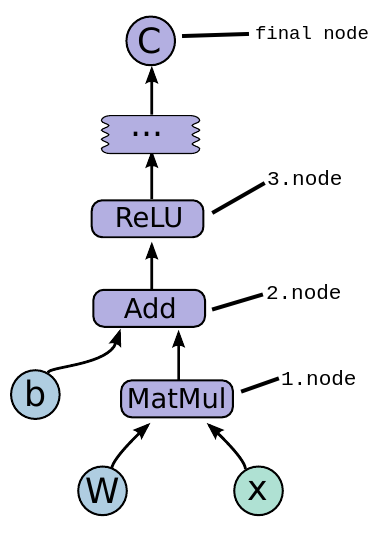
\includegraphics[width=0.25\linewidth]{graph}
\caption[placeholder]{Subgraph example of a neural network for a single neuron\footnotemark}
  \label{fig:graph_caption_placeholder_subgraph_example_for_a_neural_networkfootnotemark}
\end{figure}
\section{Execution of a Graph} % (fold)
\label{sec:execution_of_a_graph}
Each implementation follows the same standard (Fig.\ 2): Firstly, client process calls the master process through the session interface to ignite the execution. An arbitrary number of worker processes, each of which executes a subgraph, are called by the master process. Each worker is responsible for one or more devices. The number of workers depends on the architecture of the system. Master distributes the operations as well as the data tensors to the workers. Also, a worker can fetch the data by itself directly from storage system to the device's memory. Finally, the results are collected by the master and presented to the client process.
\begin{figure}[h!]
  \centering
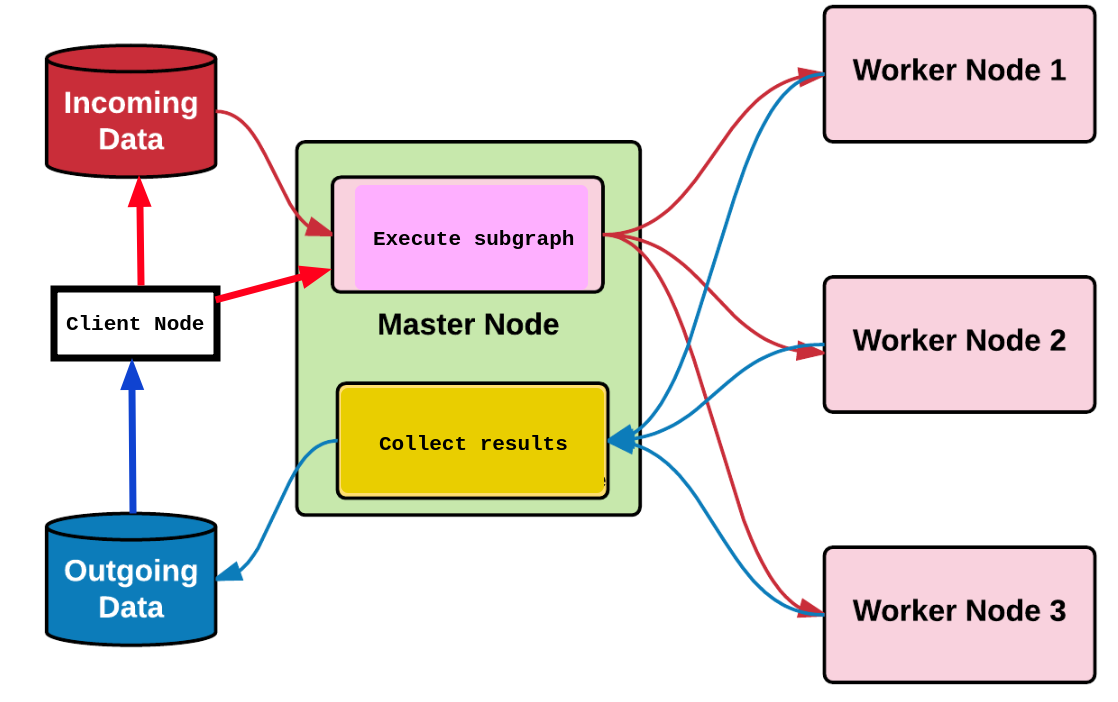
\includegraphics[width=0.5\linewidth]{executionofgraph}
 \caption[placeholder]{Master and Worker processes of a distributed system\footnotemark} 
  \label{fig:executionofgraph}
\end{figure}

\addtocounter{footnote}{-2}
\stepcounter{footnote}\footnotetext{Martin Abadi, Ashish Agarwal, ..., "TensorFlow: Large-Scale Machine Learning on Heterogeneous Distributed Systems," November 9, 2015, p.\ 3, fig.\ 2}
\stepcounter{footnote}\footnotetext{https://www.oreilly.com/api/v2/epubs/9781787281349/files/assets/Ch09-Fig11.png}

\hspace{-0.51cm}A graph can scale up immensely due to massive real-world training sets. To ensure efficiency while dealing with such graphs, we need parallelism in terms of task and data. This is why we have to utilize HPC clusters in the first place to save us a huge amount of the computation time.\ As we are going to focus on how to achieve efficiency and scalability while programming with TensorFlow on HPC systems, we first have to take a closer look at the distributed implementation of TensorFlow \cite{first}.


\section{Distributed (Multiple-Device) Implementation} % (fold)
\label{sec:multiple_device_execution_of_a_graph}
If we consider a system with a single device, the execution is fairly simple: A worker process is created for the device. Data is placed into the memory and all the nodes are mapped to the same device. The device executes them in an order according to the control dependencies between the nodes. However, in the case of an HPC system with multiple devices, we encounter a handful of programming challenges as to resource management, mapping of the nodes to the devices and intercommunication between different devices which includes any type of data transmission (e.g.\ transmitting output of a node to another node as input) required for the operation to be executed.

\subsection{Mapping of the Nodes} % (fold)
\label{sub:mapping_of_nodes}
In large-scale machine learning, we have to deal with massive data sets over thousands of petabytes. In order to train a model on such data set, hence construct a dataflow graph, we need to parallelize our node execution and also divide our data into subsets across multiple devices of our system. 
\\ \\TensorFlow uses a greedy algorithm for mapping the nodes: A cost model is prepared by estimating the size of input and output tensors for each node. Graph is traversed according to the dependencies between the nodes. For each node, the execution is simulated with the input tensors on a set of available devices which provide a kernel implementation for the respective operation. Completion time including the time for intercommunication with other devices is either measured or estimated on each device. The results are then gathered and registered on the cost model as well which contains the cost for each particular operation. Finally, the cost model is consulted to make a decision about the mapping. The device with the minimal cost is selected for the operation execution.

\subsection{Intercommunication between Devices} % (fold)
\label{sub:intercommunication_between_devices}
After the node mapping is completed, the full graph is splitted to subgraphs where each subgraph is assigned to a particular device. Due to the structure of the graph, there exist edges between the nodes which are assigned to different devices. Those edges indicate an intercommunication between the concerning devices. To handle the intercommunication efficiently, TensorFlow implements two types of nodes which are only responsible for managing the data transmission between the devices: Send-Node and Receive-Node. An edge between the devices is replaced by two edges, one from the node to Send-Node and one from Receive-Node to the other node (in Fig.3).

\begin{figure}[h!]
  \centering
  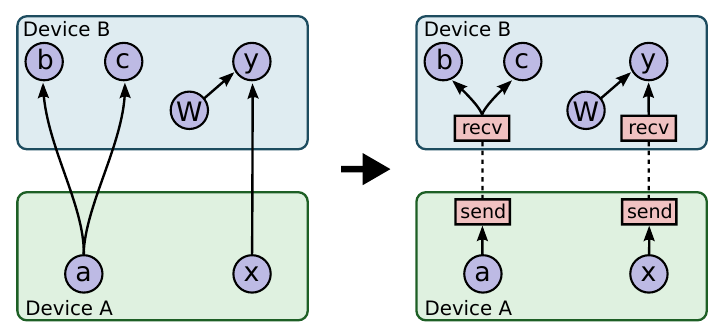
\includegraphics[width=0.5\linewidth]{intercommunication}
  \caption{Before and after replacement}
  \label{fig:intercommunication}
\end{figure}


\subsection{Ressource Management} % (fold)
\label{sub:ressource_management}





\pagebreak
\begin{thebibliography}{9}
\bibitem{first}
Martin Abadi, Ashish Agarwal, Paul Barham, Eugene Brevdo, Zhifeng Chen, Craig Citro, Greg S. Corrado, Andy Davis, Jeffrey Dean, Matthieu Devin, Sanjay Ghemawat, Ian Goodfellow, Andrew Harp, Geoffrey Irving, Michael Isard, Yangqing Jia, Rafal Jozefowicz, Lukasz Kaiser, Manjunath Kudlur, Josh Levenberg,\ldots Xiaoqiang Zheng (November 9, 2015): TensorFlow: Large-Scale Machine Learning on Heterogeneous Distributed Systems 

\bibitem{lamport94}
Leslie Lamport (1994) \emph{\LaTeX: a document preparation system}, Addison
Wesley, Massachusetts, 2nd ed.
\end{thebibliography}



\end{document}
